\chapter{Materials and Methods}
This section covers the general information for the materials and methods covered in this thesis and that are common for chapters \ref{c-invariants} and \ref{c-laser}. The methods here presented are also extended in those chapters when necessary.


\section{\textit{Lymnaea stagnalis} Neural System morphology}
\label{sec:lymnaea morphology}
The neural system of \textit{Lymnaea Stangalis} (the great pond snail) is shown in figure \ref{fig:lymn neural sys}. As in some other mollusks, e.g. {\sl Clione}, the neural system is conformed by several ganglia, each of them controlling (mainly, but not exclusively) some specific function of the snail. Figure \ref{fig:lymn neural sys diagram} shows a labeled image of the different ganglia in this system. All ganglia in the neural system are paired and distributed symmetrically, except from the visceral ganglion (unique) and the parietal, that although symmetrical, the right parietal is larger than left parietal ganglion (see \ref{fig:lymn neural sys diagram}). All ganglia are interconnected by nerves (grey stripes in the image). As mentioned before, each ganglion has an associated behavioural task in the snail. From top to bottom: we find the buccal ganglia (upper pair), which control the buccal muscle involved in the processes of open-rasp-swallow, known as the feeding cycle, initiated by a CPG circuit contained in these ganglia. The two cerebral ganglia (right bellow) are involved in the activation and modulation of many circuits and processes, including the modulation from specific neurons in all ganglia. Located on the sides of the diagram, the pedal ganglia control the snail pedal movements as crawling or swimming, and they are originally joined. The pleural ganglia, which contain sensory neurons, are connected to the mantle. And finally, at the bottom of the diagram, we find the parietal ganglion, involved in the control of the gill (respiratory organ) and the olfactory organ, and the visceral ganglion, connected to organs such as the intestine, the heart, and part of the genital system.


\begin{figure}[h!]
	\minipage{0.45\textwidth}
	\centering
	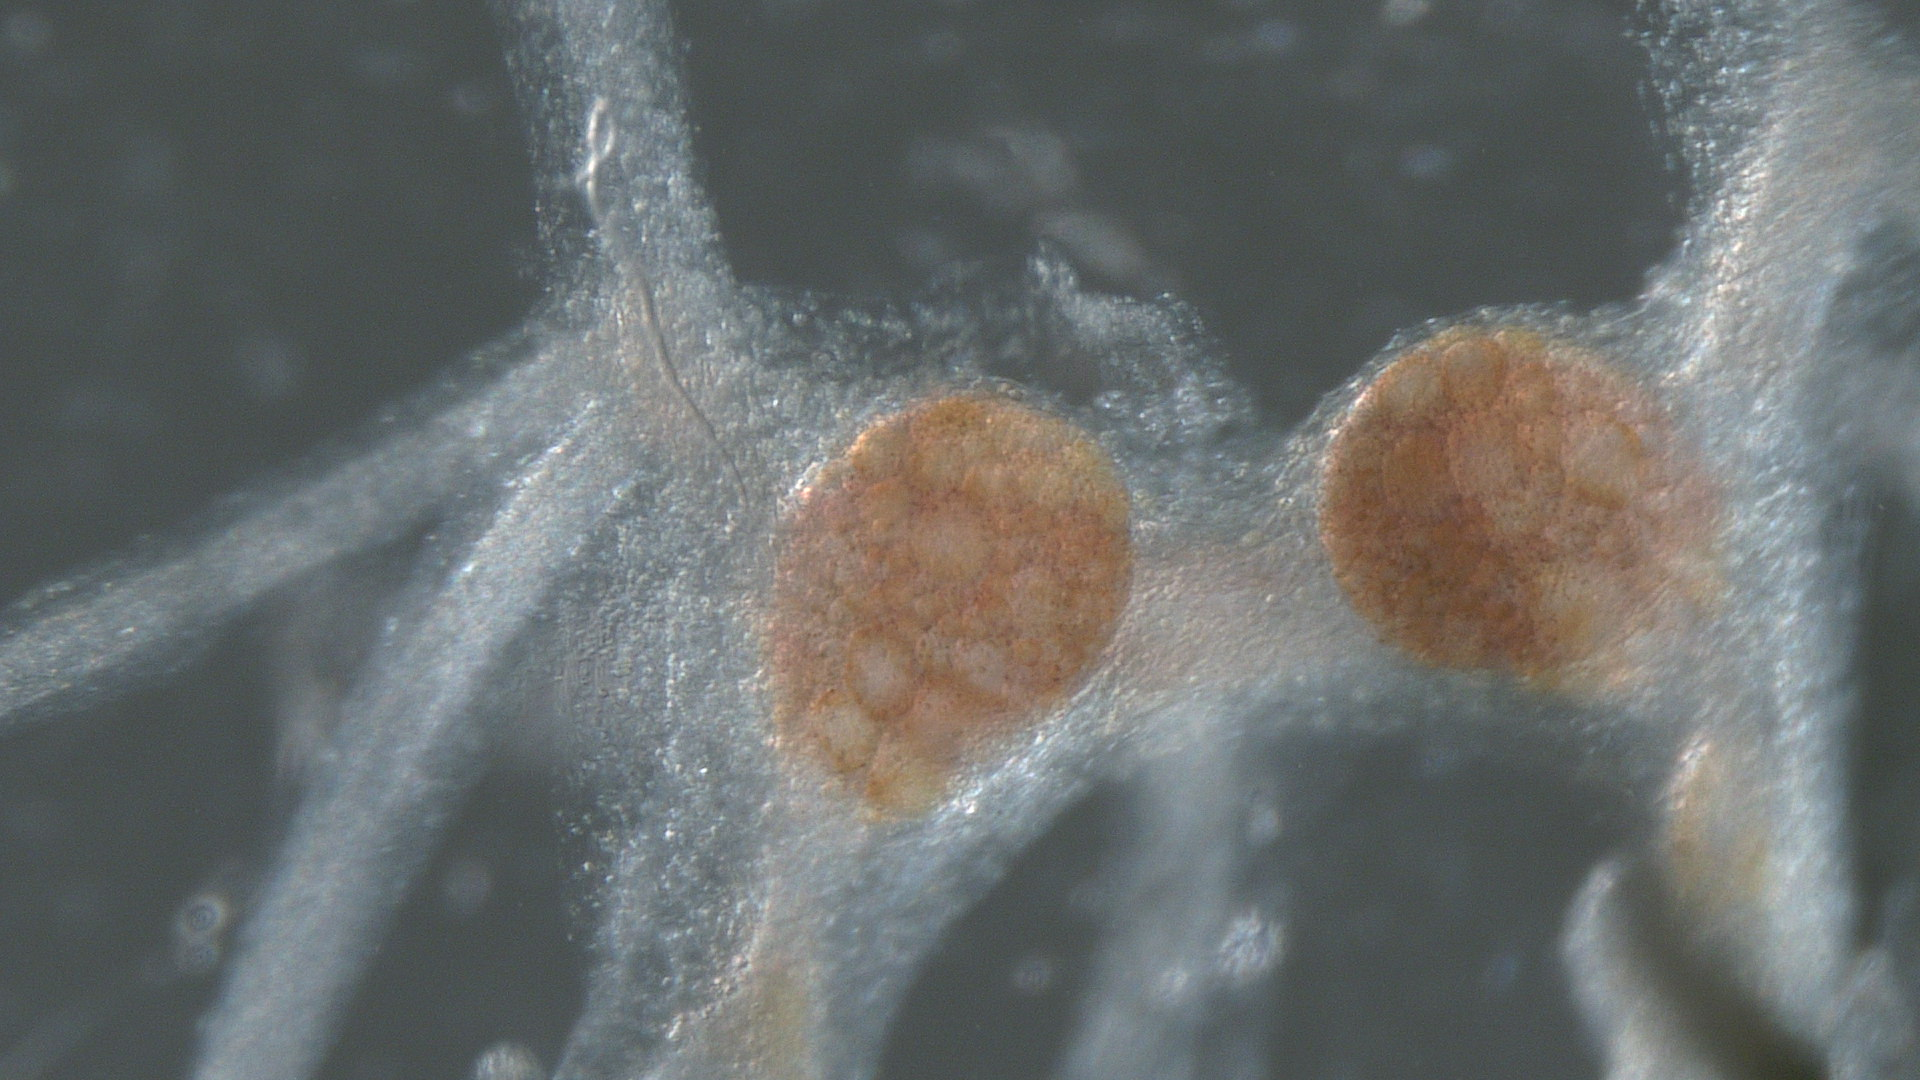
\includegraphics[angle=180,width=0.9\linewidth]{img/methods/preparation/buccal_ganglia.JPG}
	\caption{Lymnaea buccal ganglia.}
	\label{fig:buccal ganglia}
	\endminipage
	\minipage{0.45\textwidth}
	\centering
	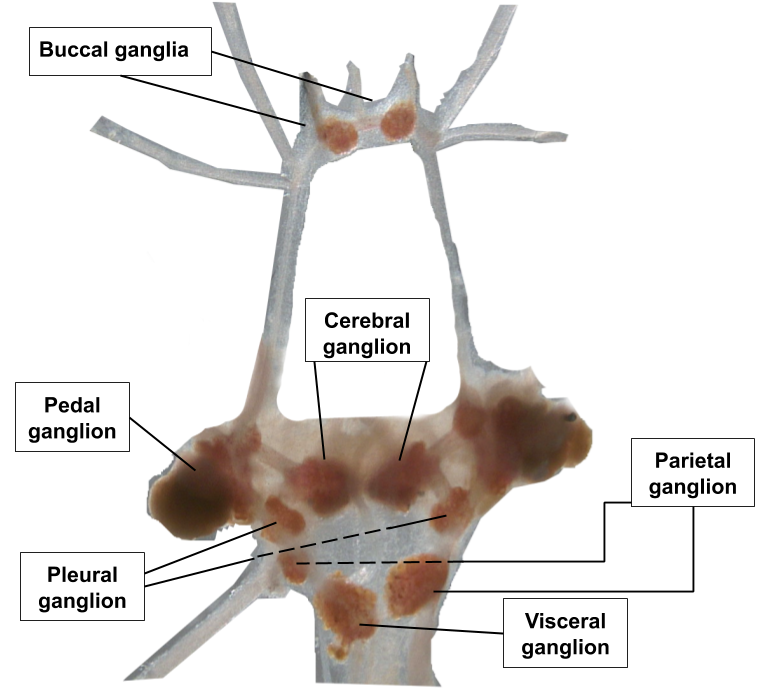
\includegraphics[width=\linewidth]{img/methods/CNS_diagram.png}
	\caption{Lymnaea nervous system diagram.}
	\label{fig:lymn neural sys diagram}
	\endminipage
\end{figure}

Neuronal recordings showed in this work are from the CPG in the buccal ganglia (see \ref{c-invariants}) and right parietal ganglia, containing large neurons with tonic firing (see \ref{c-laser}). Both ganglia are showed in detail in figures \ref{fig:buccal ganglia}.

%%%% In contrast to other systems functionality where motoneurons are CPGs neurons \cite{stomatogastric} ((page 5 review), in Lymnaea nervous system, CPGs and motoneurons are separated groups of neurons. 


\subsection{Feeding CPG in \textit{L. stagnalis}}
%
\subsection{Feeding CPG Model}
For our analysis of sequence interval variability we used the CPG model developed by Vavoulis et al. \cite{Vavoulis2007}. The model describes the activity of  three neurons conforming the CPG feeding system of the mollusk \textit{Lymnaea} (N1M, N2v and N3t cells) along with the modulator neuron SO, which has a key role in the CPG activity by regulating the feeding cycle duration. Each CPG neuron is associated to one specific movement in the feeding activity: protraction (N1M), rasp (N2v) and swallow (N3t) \cite{Benjamin2012}. During protraction, the buccal mass and radular move forwards on the food. During rasp, the radular begins to move back to get the food into the buccal cavity. During swallow, the mouth closes and the radular pushes the food into the esophagus.

The dynamics of the single neuron models are based on a Hodgkin-Huxley conductance-based formalism \cite{HODGKIN1952} describing active ionic channels with specific features to reproduce the observed waveform from experimental recordings in each cell.
The Vavoulis et al. description of the individual neurons considers a two-compartment model to represent the soma and the axon as  differentiated structures coupled by an axial resistance \cite{Vavoulis2007}. This separation of the soma and the axon is used to regulate the interaction between the fast and slow dynamics in the model. The slow dynamics are located the soma, whereas the fast dynamics are included in the axon compartment of the model. This distributed formalism is represented in Fig. \ref{fig:2 compartments}, where each circle represents either soma or axon, with a distinct ionic current distribution. The description of the compartment dynamics is provided by equations (\ref{eq:soma}) and (\ref{eq:axon}) for soma and axon, respectively: 
%Cambios
%being \(i_X\) a different channel for each neuron in the CPG (N1M,N2v,N3t).

% which is usually represented in models as \(i_{e1} = g * (V_1 - V_2)\), where $V_1$ and $V_2$ represent the voltage in each of the two compartments and $g$ is the coupling conductance, the inverse of the axial resistance and $i_{e1}$ is the current that flows into one compartment from the other.
\begin{equation}
    \tau_m\frac{dV_S}{dt} = i_{inj} - i_{L,S} - i_X - i_{ec,S} - i_{syn} \\,
    \quad with \quad i_X = [i_{ACh},i_{NaL},i_T]
    \label{eq:soma}
\end{equation}

\begin{equation}
    \tau_m\frac{dV_A}{dt} = -i_{L,A} - i_{NaT} - i_K - i_{ec,A}
    \label{eq:axon}
\end{equation}

\begin{figure}
\centering
\begin{subfigure}[t]{0.5\textwidth}
\includegraphics[width=\textwidth]{img/methods-paper-modelo/figure1a.eps} 

\caption{} \label{fig:2 compartments}
\end{subfigure}
\hfill
\begin{subfigure}[t]{0.49\textwidth}
\centering
\includegraphics[width=\textwidth]{img/methods-paper-modelo/figure1b.eps} 
%TODO FIX
\caption{} \label{fig:CPG diagram}
\end{subfigure}
 
 \caption{\textbf{Panel (a)}. Ionic channel distribution in the two-compartment description for the individual neurons in the Vavoulis et al. model \cite{Vavoulis2007} used in this study. At the soma: $I_{ACh}$, acetylcholine ionic channel; $I_{NaL}$, slowly inactivating sodium ionic channel;$I_T$, low-threshold calcium current; $I_{inj}$, injected current; $I_{L,S}$, leakage current in the soma; $I_{syn}$, synaptic current. At the axon: $I_{NaT}$, fast inactivating sodium current; $I_K$, delayed rectifier potassium current; $I_{L,A}$, leakage current in the axon. The electrical couplings are described as $I_{ec,S}=g_{ec}(V_S-V_A)$ and $I_{ec,A}=g_{ec}(V_A-V_S)$, respectively, being $g_{ec}$ the coupling conductance. The color for each $I_X$ current represents the CPG neuron that includes it at the soma,  N1M, N2v and N3t, respectively, as shown in panel (b). \textbf{Panel (b)}. Connection scheme for the {\sl Lymnaea} feeding CPG circuit model. For details on the ionic channel current descriptions and associated parameters, see \cite{Vavoulis2007}. The colors indicating each neuron in the circuit match those in the representation of their corresponding somatic membrane potential traces throughout the paper. 
}
    
    % \label{fig:2 compartments}
\end{figure}


\vspace{0.3in}

\noindent Here we follow the notation of~\cite{Vavoulis2007} where $\tau_m$ represents the time constant of the membrane (in ms) given by the ratio of the membrane capacitance (in nF) and the leakage conductance (in $\mu$S).  In equations (1) and (2), $i$ variables (given in mV) are the product of the corresponding currents (in nA) times the passive input resistance given in M$\Omega$.
%, $i=I*R$, where  $R$ is given in M$\Omega$.
% Añadir explicación de unidades********. 


The soma compartment contains a slow current $I_X$ whose ionic nature depends on the specific CPG neuron described (see Fig.~\ref{fig:2 compartments}). Thus, $I_X$  represents one channel, either $I_{ACh}$, $I_{NaL}$ or $I_{T}$, responsible of the specific slow dynamics associated with neurons N1M, N2v and N3t, respectively.  Along with the slow ionic channel and the leakage channel  $I_{L,S}$, the soma compartment also receives the synaptic current $I_{syn}$ and the injection current $I_{inj}$. All currents are explained in detail below.
%TODO al final Leakage no se pone aqui?

%A more extended explanation of these channels and the property they produce is . Along with this slow activation channels, there are also found in the soma $i_{inj}$, an injected current, and $i_{syn}$ a synaptic input that is widely explained below. These are also represented in figure \ref{fig:2 compartments}

On the other hand, fast channels are part of the axon compartment: a fast inactivating sodium current $I_{NaT}$ and a delayed rectifier potassium current $I_{K}$. These channels, along with the axon leakage channel  $I_{L,A}$ are also represented in Fig.~\ref{fig:2 compartments}, for their detailed description see~\cite{Vavoulis2007}. 


% ***Descripción breves de corrientes en terminos de cuales son lentas y rápidas con referencia a la Fig.1
% y la i_x

The model cells as described above are not endogenously bursters. To achieve a realistic bursting activity in each neuron, a distinct constant value of  \(i_{inj}\) is applied to the cells. %  Values of \(i_{inj}\) used in this study to obtain realistic bursting activity. 
%TODO añadir " in the circuit".

 The CPG topology scheme is shown in Fig. \ref{fig:CPG diagram}, where the connections between neurons are represented by dashed or solid lines, depending on whether the connection is slow or fast, respectively, and filled or empty circles at their end denoting the direction and the effect on the postsynaptic neuron: excitation (empty circles) or inhibition (filled circles).
Individual neurons following the previous description are connected by graded synapses, defined by equations (\ref{eq:syn1}-\ref{eq:syn2}) \cite{Vavoulis2007}:

% \begin{equation}
%     i_{syn} = \sum_j \gamma_{syn,j} s_j (V_S - E_{syn,j})
%   \label{eq:syn1}
% \end{equation}
% % TODO FIX
% \begin{equation}
%     \frac{ds_j}{dt} = \frac{r_{j}-s_j}{\tau_{syn,j}}
% \end{equation}

% \begin{equation}
%   \frac{dr_j}{dt} = \frac{r_{\infty,j}-r_j}{\tau_{syn,j}}
% \end{equation}

% \begin{equation}
%     r_{\infty,j}=\frac{1}{1+e^{(-40-V_{pre_{V_S}})/2.5}}
%      \label{eq:syn2}
% \end{equation}


\noindent where index $j$ runs over all presynaptic neurons and \(\gamma_{syn,j}, E_{syn,j},\tau_{syn},V_{pre_{V_S}}\) are the product of input resistance and maximal synaptic conductance, the synaptic reversal potential, the synaptic time constant and the presynaptic potential, respectively.
%cambio

Together with the effect of the distinct connections conforming the circuit, the neuron dynamics in this model is shaped by the ionic channels at each cell and their associated parameters. The resulting triphasic CPG rhythm with distinct voltage waveforms of spiking-bursting activity is displayed in Fig. \ref{fig:model simulation}, where the effect of the connections in building the phase between neurons can also be observed. The traces correspond to a simulation of the complete circuit model, i.e., all connections shown in Fig. \ref{fig:CPG diagram} are active. 


\begin{figure}[h!]
    \centering
    \includegraphics[width=\linewidth]{img/methods-paper-modelo/figure2.eps}
    \caption{Triphasic feeding rhythm as produced by the circuit CPG model described in Fig. \ref{fig:CPG diagram}. In this simulation, $i_{inj}$ values applied to each neuron are 8.5, 6, 2 and 0 mV, respectively.}
    \label{fig:model simulation}
\end{figure}

The distinct waveforms for each neuron are mainly due to their specific ionic channel dynamics. On the one hand, N1M voltage characteristics are provided by an acetylcholine sensitive channel (\(i_{ACh} = 200 * p^3 * (V_S + 30)\)), which causes the gradual spiking frequency increase as well as the visible plateau, i.e., the slow wave is sustained before hyperpolarization. On the other hand, N2v has a slowly inactivating sodium channel (\(i_{NaL} = 2 * p^3 * q^3 * (V_S-55)\)), which causes the slow depolarization in this neuron. N2v neuron has a lower spiking frequency caused by the conductance value given for the axial $g_{ec}$ linking the two compartments, which is much lower in this cell. Finally, the N3t neuron has the particularity of a post inhibitory rebound, which generates an initial fast spiking followed by a decrease in the firing rate as the burst evolves. This latter property is caused by a low-threshold calcium channel (\( i_T = 3.27 * p^3 * q *(V_S-80)\)).

%cambios
In contrast to the N1M, N2v and N3t neurons of the CPG, the model of the SO neuron has no \(I_X\) channel, so its activity is the result of the combination of the common ionic channels in the axon and the soma.
% ****no se dice nada de la SO ****

\subsection{Inducing variability by current injection}
\label{subsec:inj protocol}
The spiking-bursting activity of the model CPG neurons can be modulated by using an additional current injection on each cell, implemented in the \(i_{inj}\) term of equation (\ref{eq:soma}), as performed in many experimental protocols. Depending on the value % of the current 
applied,%TODO current o value applied?
% the corresponding neuron dynamics changes. While for N2v a change in this current injection corresponds to a change in burst frequency (i.e. the number of bursts increases/decreases), for the rest of the neurons in the model (N1M, N3t and SO) a change in \(i_{inj}\) affects their burst duration. %%TODO ????
the corresponding neuron dynamics changes. While for N2v a change in this injection corresponds to a change in burst frequency (i.e. the number of bursts increases/decreases),
for the rest of the neurons in the model a change in \(i_{inj}\) affects burst duration for N3t and SO,  and the length of the depolarization phase in N1M.


Whilst the single neuron model descriptions have no intrinsic variability, the effect produced by the modulation of the injected current in each neuron induces variability into the circuit, which allows characterizing the sequence intervals and the period, the associated robustness of the rhythm and the presence of dynamical invariants. Such stimulation has been used previously in the living circuit, as reported by Elliot et al. \cite{Elliott1991}. The authors of this work showed that it is possible to activate the feeding CPG with variability caused by current injection into individual cells in the circuit. CPG rhythms obtained under this type of stimulation differ depending on which neuron is being stimulated. 

% Even though this CPG model do not present intrinsic variability, thanks to the current \(i_{inj}\), variability is induced into the model, effectively changing burst duration. This current injection has also been used in Lymnaea preparation in living elements, stimulating N1M and SO, obtaining rhythm. Neural sequences obtained after the stimulation differ one another depending on which neuron is being stimulated. 

By varying the current injected into N1M, its burst duration is kept nearly constant, but its depolarization phase before the spiking activity begins becomes longer. Since N3t is the neuron fitting in the sequence in that phase (see Fig. \ref{fig:model simulation}), it also increases its burst duration, being the most variable one in the CPG rhythm. 

When %current 
value \(i_{inj}\) is increased on neuron SO, its burst duration becomes longer. Since SO has a modulator effect over N3t and N1M, it also alters the burst duration of these two neurons.

Neuron N3t also shows variable burst duration when an evolving current is injected. When \(i_{inj}\) increases on N3t, its burst duration increases, elongating the N1M depolarization phase.  

Finally, when current is applied to N2v the effect on its burst duration or the burst duration of the rest of the neurons is rather small. However, \(i_{inj}\) % current 
modulates N2v burst frequency through the hyperpolarization phase. 

%cambios
Therefore, we used a current ramp protocol to induce variability in the CPG model defined as follows: a ramp variable $c$, which controlled the current injection value ($i_{inj}=c$) %TODO
on the neuron being stimulated, was increased from a minimum to a maximum value, and then decreased back to the initial value. This was repeated twice in each simulation. The ramp variable was modified with a fixed step value every 4.6 seconds (the approximate duration of two N3t bursts).
% occurrence of each two bursts in N3t neuron (every 5 seconds). ***discutimos esto, es cada burst o cada dos como dice abajo, quizás convendría decir que corresponde a ese tiempo en el modelo sin estímulo. Por otro lado el lector se podría preguntar por qué no es una rampa de subida y bajada prestablecida en el tiempo***
The minimum and maximum $c$ values were different in each cell and were %chosen experimentally using model simulations 
tuned to generate realistic spiking-bursting behavior. %cambios : añadir por si experimentally no se entiende bien? depending on the effect of the injected current on the neuron to ensure robust burst generation in all neurons 
%Note that this variable $c$ value which goes through the different values in the ramp is $i_{inj}$ value, replacing the constant value of this current.
All parameters used for the simulation analyses reported in this paper are summarized in Table \ref{table:inj values}. An example of how this ramp current injection affects the rhythm is shown in Fig. \ref{fig:complete ramp example}. 
%cambios : quitar esta frase e indicarlo en seccion 2.3
% The rest of model and synapse parameters used to simulate the model are the same ones specified in the paper that describes the Vavoulis et al. model \cite{Vavoulis2007}.


\begin{table}[h!]
\centering
\begin{tabular}{c|cccc|c|ccc|}
\multirow{2}{*}{\textbf{\begin{tabular}[c]{@{}c@{}}Neuron\\ stimulated\end{tabular}}} & \multicolumn{4}{c|}{\textbf{\(i_{inj}\) value}}                 & \multirow{6}{*}{} & \multicolumn{3}{c|}{\textbf{Ramp values ($c$)}}   \\ \cline{2-5} \cline{7-9} 
                                                                                      & \textbf{SO} & \textbf{N1M} & \textbf{N2v} & \textbf{N3t} &                   & \textbf{Min} & \textbf{Max} & \textbf{Step} \\ \cline{1-5} \cline{7-9} 
\textbf{N1M}                                                                          & 8.5         & $c$            & 2            & 0            &                   & 0            & 10.5         & 0.5           \\ \cline{1-5} \cline{7-9} 
\textbf{N3t}                                                                          & 9           & 10           & 1            & $c$            &                   & 0            & 5            & 0.25          \\ \cline{1-5} \cline{7-9} 
\textbf{SO}                                                                           & $c$           & 10           & 1            & 4            &                   & 8.2          & 13           & 0.25          \\ \cline{1-5} \cline{7-9} 
\end{tabular}
\caption{List of \(i_{inj}\) values that yield realistic bursting rhythms for each neuron in the model CPG used in the stimulation protocols reported in this paper. The left section of the table displays the \(i_{inj}\) values applied to each neuron (columns) during each simulation condition (rows). Ramp values on the right section refer to the minimum and maximum values of the ramp variable $c$ in each simulation, increasing \(i_{inj}\) in the specified step every 4.6 seconds (the approximate duration of two N3t burst) to induce variability.} \label{table:inj values}
\end{table}


\begin{figure}[h!]
    \centering
    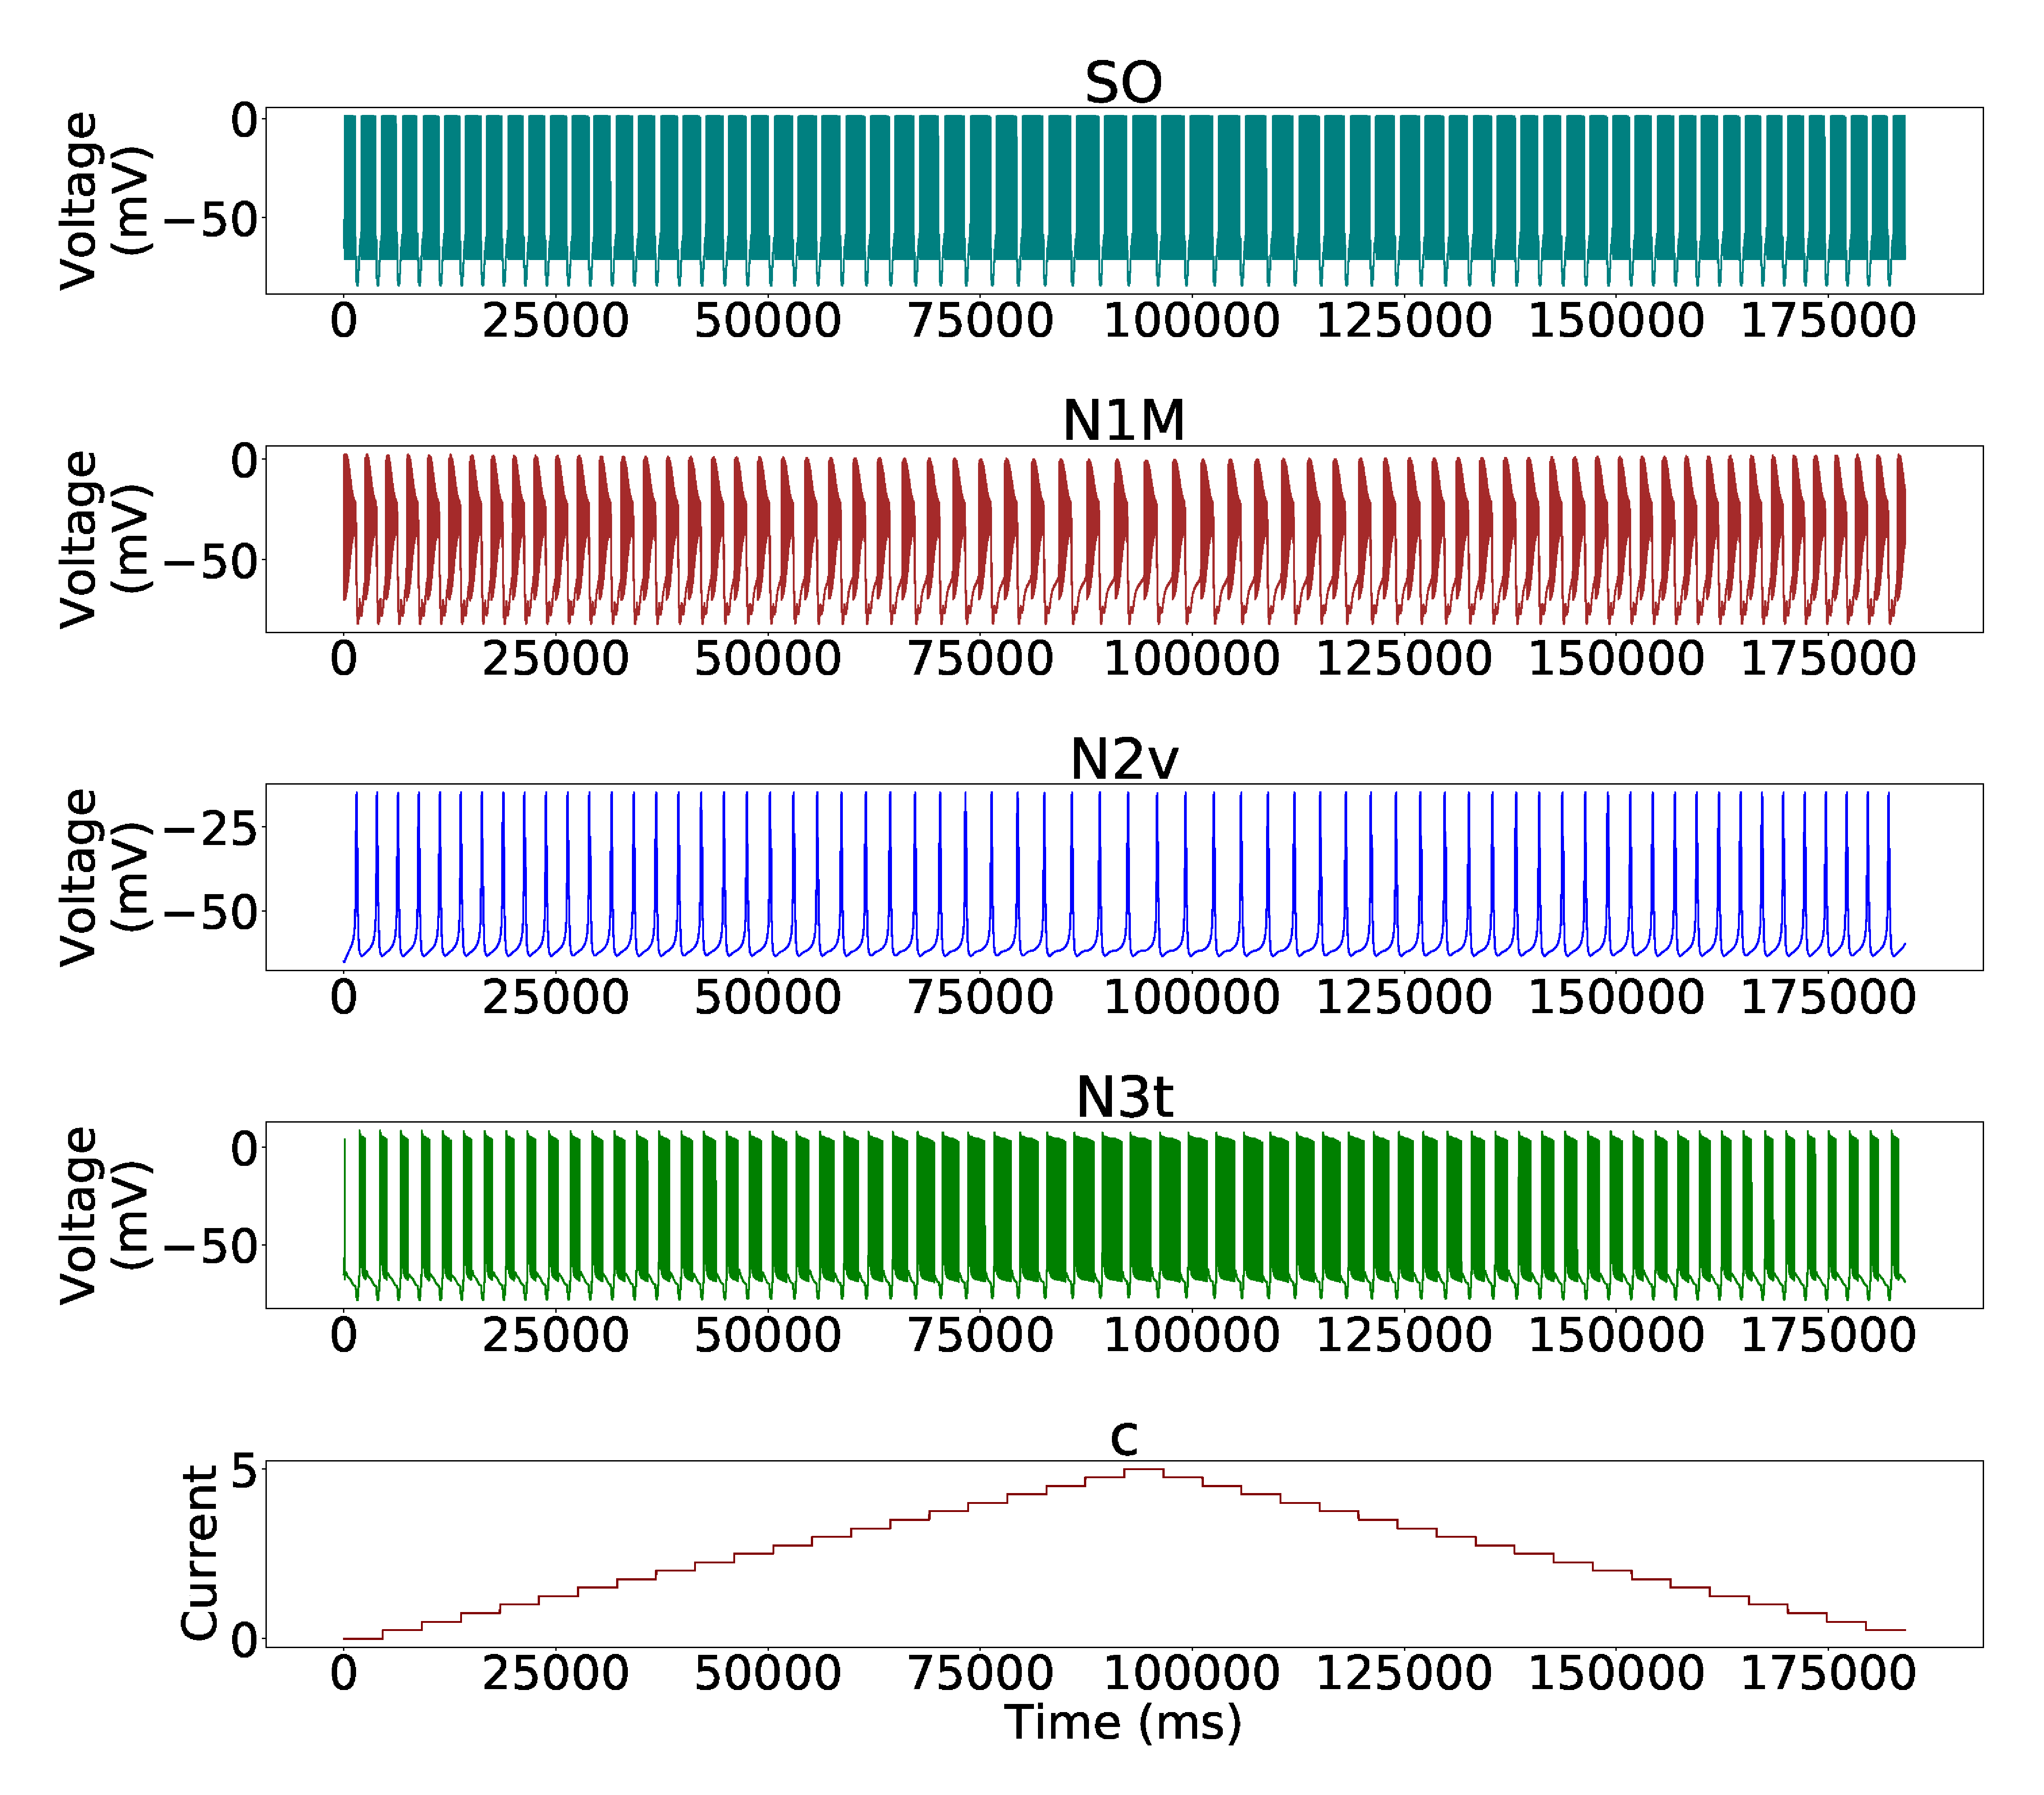
\includegraphics[width=\textwidth]{img/methods-paper-modelo/figure3.eps}
    \caption{Illustration of the CPG activity when a current ramp \(i_{inj}\) is applied to N3t. Variability in the sequence intervals was induced by applying two consecutive ramps as the one shown in this figure into different cells.  }
    \label{fig:complete ramp example}
\end{figure}


\subsection{Model simulation specifications and statistical analysis}
Simulations of the Vavoulis et al. model \cite{Vavoulis2007} were implemented in C++. The code of the feeding CPG model implementation is available at \url{https://github.com/GNB-UAM/CPG-feeding-Lymnaea}. Each simulation had the duration of two consecutive cycles of up and down ramps as the one shown in Fig. \ref{fig:complete ramp example} using the parameters described in Table \ref{table:inj values}. The number of bursts in each simulation was approximately 140 (this number slightly depends on the neuron stimulated). Parameter values such as reversal potentials and synaptic conductances were the same ones specified in \cite{Vavoulis2007}.
The statistical analysis was done in Python 3.6. For the temporal variability study, first the spikes were detected %\sout{using a threshold protocol. Due to the drift in the spike amplitude during the bursting of some of the neurons (as N2v), the spike detection was performed over the $1^{st}$ derivative of the signal}
using the change in the derivative during the computation of the model along with a threshold condition. Then, bursts were identified from the temporal structure of the spikes, and intervals were characterized by the timing of the first and last spike in each burst. 

Thus, all intervals defined below in section \ref{subsec:intervals} were measured and their variability was characterized by statistical analysis tools, i.e,  boxplots and linear correlations. For the boxplots, the Python library matplotlib.pyplot used each cycle-by-cycle interval duration. Linear regression from sklearn Python library was used to quantify the relation of the sequence intervals to the instantaneous period of each cycle. 

\subsection{Time references, intervals and CPG sequence}
\label{subsec:intervals}
The variability study addressed here is based on the characterization of  cycle-by-cycle intervals in the rhythm produced by the model CPG. % In order to explore possible dynamical invariants on this \textit{Lymnaea} feeding CPG, the intervals here analyzed follow the ones defined for the stomatogastric CPG dynamical invariants \cite{Elices2019}. Hence, based on the burst duration we will have in each cycle all corresponding burst duration intervals and some derived intervals obtained by the combination of pair of neurons, as well as the period. The resulting intervals here analyzed are shown in figure \ref{fig:intervals}. 
In our analysis of variability, we assess the presence of linear relationships between the intervals that build the sequence and the cycle-by-cycle period to characterize and unveil similar dynamical invariants as those found in the stomatogastric CPG \cite{Elices2019}. 
%Hence, we characterize the intervals building the CPG sequence, including its period. 
%on the burst duration we will have in each cycle all corresponding burst duration intervals and some derived intervals obtained by their combination of pair of neurons, including the period.
% Hence, the burst events detected are going to be used to define three intervals in the trace of each individual neuron, and two additional intervals defined from the relation between two neurons. 
This is illustrated in Fig. \ref{fig:intervals}, where single neuron intervals and intervals defined between neurons are depicted. 
%cambios
The intervals here analyzed can be measured for any three neurons following a robust triphasic rhythm. In this paper N1, N2 and N3 represent the feeding CPG neurons simulated in the model: N1M, N2v and N3t, respectively.

% Here is the definition of each interval:
% \begin{enumerate}
%     \item \textbf{Burst Duration (BD)}, measured as the time interval between the first and the last spike of the burst (start to end in the trace of a given neuron).
%     \item \textbf{Inter burst interval (IBI)}, characterised as the difference between the last spike of a burst and the first one of the next one (end to start in the trace of a given neuron).
%     \item \textbf{Period}, which envelops the bursts from the three neurons, measured as the distance between the first spike of one burst in a neuron and the first spike of the next one on that neuron (start to start).
%     \item \textbf{NeuronX-NeuronY interval}, this interval is measured from the burst beginning of neuron X to the burst beginning of neuron Y (start X to start Y).
%     \item \textbf{NeuronX-NeuronY delay}, being the time lapse between the burst end of a neuron X and the burst beginning of neuron Y. (end X to start Y).
% \end{enumerate}

\begin{figure}
\centering
\begin{subfigure}[t]{\textwidth}
\centering
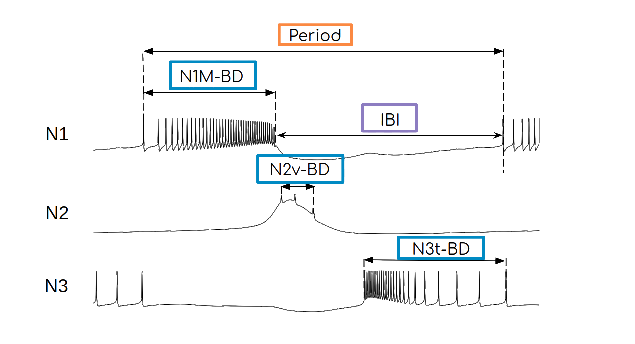
\includegraphics[scale=0.8]{img/methods-paper-modelo/figure4a.eps} 
\caption{} \label{fig:intervals_bd}
\end{subfigure}
% \hfill

    \vspace{1cm}
\begin{subfigure}[t]{\textwidth}
\centering
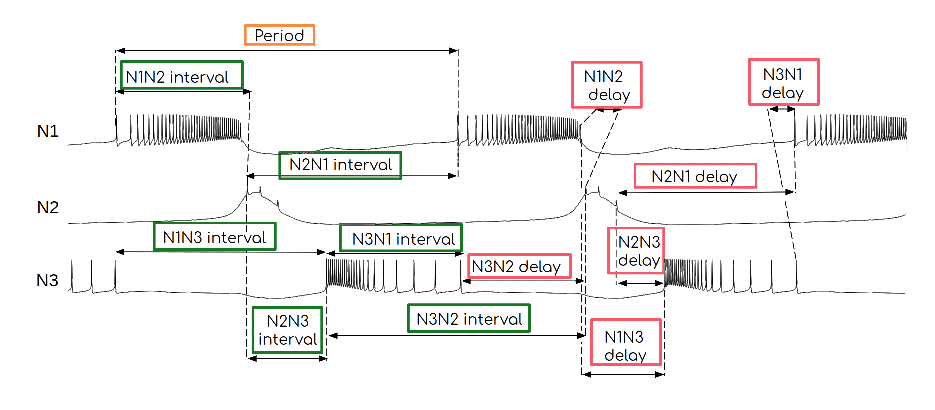
\includegraphics[scale=0.8]{img/methods-paper-modelo/figure4b.eps} 
\caption{} \label{fig:intervals_der}
\end{subfigure}
 
 \caption{\textbf{Panel A}. Individual neuron sequence interval definitions. Each BD label represents the burst duration, defined as the time interval from the first spike to the last spike in the neuron's burst. Period was measured as the interval from the first spike of N1 burst to the first spike of the next N1 burst, covering three phases %(N1M,N2v, N3t) 
 in relation to the activity of the other neurons. IBI represents the interburst interval, defined as the time from the last spike of a neuron's burst to the first one of the next burst in the same neuron.
    \textbf{Panel B}. Definition of intervals involving pairs of neurons. NXNY interval represents interval from NX start to NY start. NXNY delay represents interval from NX end to NY start. Period was measured from N1 start to N1 start, covering the three phases of the CPG rhythm.
    }
    
    \label{fig:intervals}
\end{figure}

\clearpage
\newpage



% ***quizás convendría añadir una subsección en los métodos diciendo cuál es la duración de las series temporales, las ráfagas que contienen y que se detectan los spikes para caracterizar los intervalos ciclo a ciclo. También que la variabilidad se caracerizó con boxplots del coeficiente de variación de todos los intervalos. Las figuras de los boxplots no parecen en porcentajes, los valores negativos habría que explicarlos en términos de que la fase de algunas neuroans se adelanta con respecto a lo definido en la figura 4 ***


%For the purpose of this study, the nerves employed for the extracellular recordings are the symmetrical pair of nerves coming out from the buccal ganglia, which were originally connected to the buccal mass. Since these nerves send out the impulses to move the muscles, the neurons whose activity is recorded in the extracellular signals are mostly motoneurons \cite{Benjamin1979a}, not the ones initiating the rhythm but the ones following the CPG neurons. It is important to localize these neurons in the extracellular recording for detecting the rhythm and the patterns. 
% On the one hand, the feeding rhythm in \textit{Lymnaea} is pretty slow and it is not always active. 

\subsubsection{Lymnaea feeding rhythm}

The feeding activity of the \textit{Lymnaea}, concerning the buccal mass, is classified in three main steps: Rest, protraction, rasp and swallow. This sequence of buccal movements in the snail is generated by the motor neurons distributed in the ganglia. Each of these phases is leaded by one interneuron from the CPG: N1M, N2v, N3t, and followed by the motoneurons associated to them. This is a complex distributed system where motoneurons do not exclusively follow the interneurons but are also implied in the feeding cycle activation \cite{staras_pattern-generating_1998}. In this circuit there are also some modulatory neurons implied such as SO neuron (in the same buccal ganglia) or CGC (in the cerebral ganglia). 

Hence, an initial resting state, where the CPG as well as the moto-neurons have no activity, may change due to a sensory input. This input, received in the presence of food or during hunger, is handled in the cerebral ganglia generating activity and changing the SO tonic spiking during resting (which was inhibiting the CPG) to a bursting mode, meaning the start of the feeding cycle.


This CPG circuit can be studied in a disected preparation, since snail's neurons are active after the isolation of the system. Specially, the CPG rhythm is maintained after its activation and it is generated in an autonomous way by the neurons in the circuit. However, due to the slow dynamics of the system and the nature of the experimental setting there are different ways to initiate the rhythm. In \textit{Lymnaea} literature, several options are proposed to solve this issue. The first solution is stimulating the neurons responsible for the initiation of the feeding rhythm, such as the SO modulator neuron on the buccal ganglia or also the CBC, CVs neurons, located on brain ganglia. Stimulating these cells usually activates the target circuits \cite{benjamin_distributed_2012}. However, the access to these neurons is not always easy and it might be necessary to keep them in constant stimulation. Another option for activation discussed in the literature is appliying octopamine. Some neurons in the buccal ganglia are sensitive to octopamine and, as a result, this procedure activates the rhythm \cite{vehovszky_octopamine-containing_2004}. Alternatively, in a semi-intact preparation, it can be applied sucrose to activate the rhythm \cite{vavoulis_computational_2007,vehovszky_octopamine-containing_2004,straub_endogenous_2002}. As a foresighted option, controlling the snails' feeding and selecting the first animal approaching the food seems to be effective for obtaining the feeding rhythm, with up to 80\% of success \cite{Elliott1991}.\todo{del tfm, quitar?}




\section{Electrophysiology in \textit{Lymnaea Stagnalis}}

\label{subsec:preparation}
In this thesis, intraceullular neuronal recordings have been carried out in the mollusk \textit{Lymnaea Stagnalis}. Beyond the advantages of invertebrates discussed in section \ref{c-intro-invertebrates} -- its easy accessible neural system, the size and resistance of its neurons to electrode impaling, the great pond snail's neural system is detailed described and so it is the feeding CPG which has been the model of study for chapter \ref{c-invariants} in this work. Also its slow dynamics, are convenient when studying the sequential evolution of the modulation, as in the case of the laser stimulation described along chapter \ref{c-laser}. 

The technique followed for the neural activity acquisition was intracellular recordings with filled with 3 M $KCl$ sharp electrodes, % in Figure \ref{fig:membranepotential recording} there is a scheme of the potential measurement. Está en la intro.
 In this technique, a glass micropippete penetrates the cell to record its activity, with a minimal damage on the cell, and the membrane potential is then recorded using a DC amplifier (ELC-03M, NPI Electronic, Hauptstrasse, Tamm, Germany). Micropippetes were pulled using a Sutter Instruments puller (Model P-97) (see Figure \ref{fig:electrode}). Membrane potential was recorded and recordings were acquired at 10 KHz using an A/D board (PCI-625 with a BNC-2090A DAQ device, National Instruments).

To facilitate the access to the cell, the sheath above it was reduced using protease (Sigma XVII) over the ganglion for $\sim$1 min and then washed with fresh saline. In order to record cell signals extra- and intracellularly, it is necessary to have full access to the neural system. Although there is an option to keep the buccal mass and do a semi-intact preparation \parencite{staras_cellular_1999} in this work the neural system (ganglia and nerves) was fully isolated (see \cite{garrido-pena_tfm_2022} for more details). The preparation was immersed in a saline solution (in mM: 51.3 $NaCl$, 1.7 $KCl$, 1.5 $MgCl_2\cdot6H_2O$, 4.1 $CaCl_2\cdot2H_2O$, 5 $HEPES$, corrected to pH 7.8 with 4 $M$ $NaOH$). All procedures followed the European Commission and Universidad Autónoma de Madrid animal treatment guidelines.

\begin{figure}[hbt!]
	\centering
	\begin{minipage}{0.4\textwidth}
		\centering
		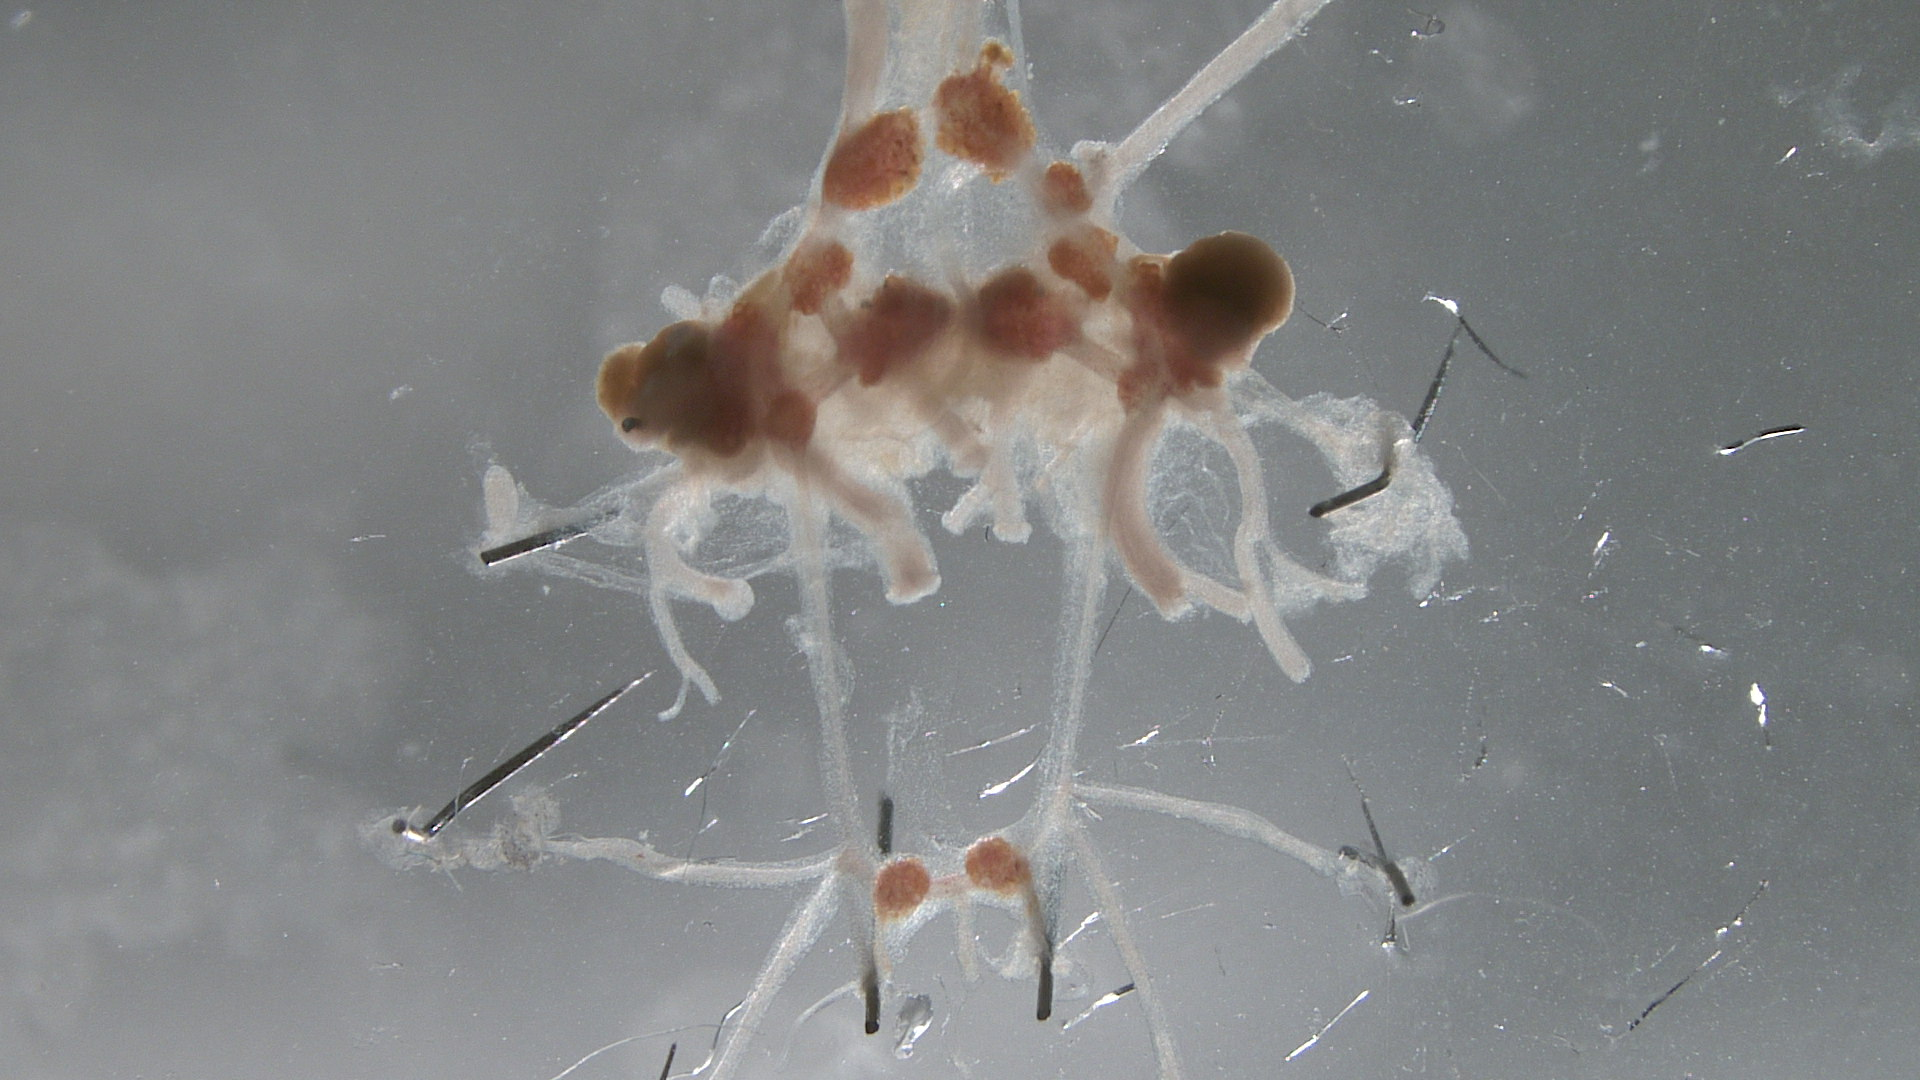
\includegraphics[angle=180,width=0.99\linewidth]{img/methods/IMG00027.jpg}
		\caption{\textit{Lymnaea stagnalis} neural system isolated.}
		\label{fig:preparation}
	\end{minipage}
	\hfill
	\begin{minipage}{0.4\textwidth}
		\centering
		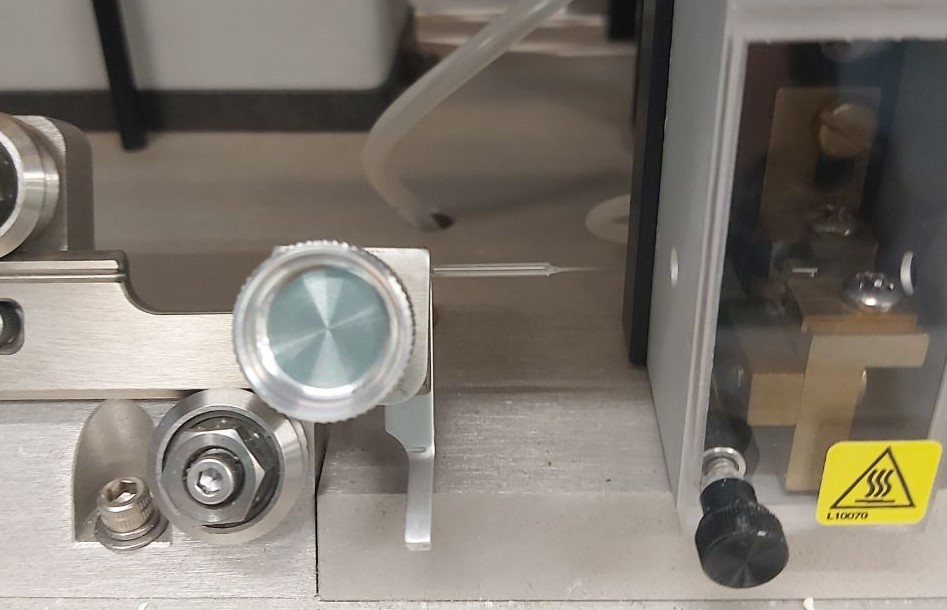
\includegraphics[width=0.99\linewidth]{img/methods/preparation/electrode4_zoom.jpg}
		\caption{Example of a sharp micro-electrode glass}
		\label{fig:electrode}
	\end{minipage}
\end{figure}


\section{Conductance based models}
For the theoretical analyses in this work, there have been used simulations of conductance-based models. As discussed in section \ref{computational neuroscience}, these models are based on a specific combination of ionic channels with a dynamic dependent on time that reproduces the Voltage value in the membrane at each time instant. There are many types of models and descriptions, depending on the specific combination of channels. Models used in this work, for both chapters \ref{c-invariants} and \ref{c-laser}, are description of neurons in \textit{Lymnaea stagnalis} for a neuron in cerebral ganglia, CGC \parencite{vavoulis_balanced_2010} and neurons in the feeding CPG in the buccal ganglia --SO, N1M, N2v, N3t, \parencite{vavoulis_computational_2007}. The first one, simulates a tonic firing and shoulder shape spike waveform, similar to the activity in some neurons in the right parietal ganglion. The second model is a detailed description of the CPG circuit with a combination of two-compartments neurons and a gradual synapse, that allows sufficient flexibility in the circuit to induce variability in the model --this will be discussed in detail in section \ref{c-invariant-models}. Equations \ref{eq:CGC}-\ref{eq:synapse} describe these to models. 

\subsection{CGC neuron model}
 This model is described by six different ionic channels: Persistent and transient sodium currents ($I_{NaP}$, $I_{NaT}$); transient and delayed rectifier potassium currents ($I_A$, $I_D$), and a low-voltage-activated and high-voltage-activated calcium currents ($I_{LVA}$, $I_{HVA}$), described by Eqs. \ref{eq:voltage} to \ref{eq:channels}. \todo{añadir para qué es cada corriente}
 
  \begin{equation}
 	C_m\frac{dV}{dt} = I_{inj} - I_{NaT} - I_{NaP} - I_{A} - I_{D} - I_{LVA} - I_{HVA},
 	\label{eq:voltage}
 \end{equation}
 
 \begin{equation}
 	I_{NaT} = g_{NaT} m_{{\infty}}^3 h (V - E_{Na}),
 \end{equation}
 \begin{equation}
 	I_{NaP} = g_{NaP} r^3 (V - E_{Na}),
 \end{equation}
 \begin{equation}
 	I_{A} = g_{A} a^4 b (V - E_{K}),
 \end{equation}
 \begin{equation}
 	I_{D} = g_{D} n^4 (V - E_{K}),
 	% \label{eq:channels}
 \end{equation}
 \begin{equation}
 	I_{LVA} = g_{LVA} c_{{\infty}}^3 d_{{\infty}} (V - E_{Ca}),
 \end{equation}
 \begin{equation}
 	I_{HVA} = g_{HVA} e^3 f (V - E_{Ca}).
 	\label{eq:channels}
 \end{equation}

Inactivation and activation dynamic variables $r,a,n,e$ and $h,b,f$ are defined by:
\begin{equation}
	\frac{dx}{dt} = \frac{x_{\infty}-x}{\tau_x},
	\end{equation}
where $x = h,r,a,b,n,e$ or $f$ and $x_{\infty}$ and $tau_x$ are defined by:

\begin{equation}
	x_{\infty} = {(1+exp(\frac{V_H^x-V}{V_S^x}))}^{-1}
\end{equation}

See Supplementary Material in \cite{vavoulis_balanced_2010} for more details. 

The implementation of this model is available at Neun library \href{https://github.com/GNB-UAM/neun}{github.com/GNB-UAM/neun} (VavoulisCGCModel).

\begin{figure}[htb!]
	\centering
	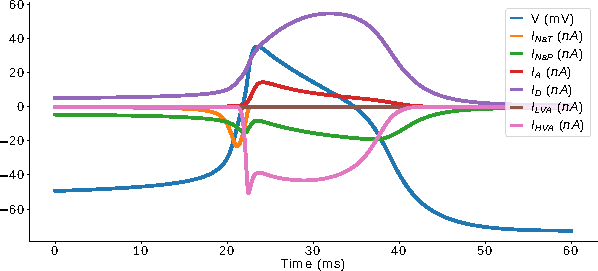
\includegraphics[width=\textwidth]{img/laser/cgc-model-simulation.pdf}
	\caption{Simulation of the CGC-model representing the voltage dynamics during an action potential and the corresponding ionic currents defined in the model ($I_{\textrm{NaP}}$,$I_{\textrm{NaT}}$, $I_{\textrm{A}}$, $I_{\textrm{D}}$, $I_{\textrm{LVA}}$,$I_{\textrm{HVA}}$). The units in the $y$-axis are specified in the legend.}
\end{figure}

\subsection{Feeding CPG model}
The Vavoulis et al. description of the individual neurons considers a two-compartment model to represent the soma and the axon as  differentiated structures coupled by an axial resistance \cite{Vavoulis2007}. This separation of the soma and the axon is used to regulate the interaction between the fast and slow dynamics in the model. The slow dynamics are located the soma, whereas the fast dynamics are included in the axon compartment. This distributed formalism is represented in Fig. \ref{fig:CPG diagram 2 compartments}a., where each circle represents either soma or axon, containing the different ionic currents for each one. The description of the voltage dynamics is provided by equations (\ref{eq:soma}) and (\ref{eq:axon}) for soma and axon compartments, respectively: 

\begin{equation}
	\tau_m\frac{dV_S}{dt} = i_{inj} - i_{L,S} - i_X - i_{ec,S} - i_{syn} \\,
	\quad with \quad i_X = [i_{ACh},i_{NaL},i_T]
	\label{eq:soma}
\end{equation}

\begin{equation}
	\tau_m\frac{dV_A}{dt} = -i_{L,A} - i_{NaT} - i_K - i_{ec,A}
	\label{eq:axon}
\end{equation}


\begin{figure}
\centering
\begin{minipage}[t]{0.45\textwidth}
	\raggedright
	(a) \par
	\vspace{75pt}
	\includegraphics[width=\textwidth]{methods/invariants-model/figure1a.eps}
\end{minipage}\hfill
\begin{minipage}[t]{0.45\textwidth}
	\raggedright
	(b) \par
	\includegraphics[width=\textwidth]{methods/invariants-model/figure1b.eps}
\end{minipage}
	\caption{\textbf{Panel (a)}. Ionic channel distribution in the two-compartment description for the individual neurons in the Vavoulis et al. model \cite{Vavoulis2007} used in this study. At the soma: $I_{ACh}$, acetylcholine ionic channel; $I_{NaL}$, slowly inactivating sodium
		ionic channel;$I_T$, low-threshold calcium current; $I_{inj}$, injected current; $I_{L,S}$, leakage current in the soma; $I_{syn}$, synaptic current. At the axon: $I_{NaT}$, fast inactivating sodium current; $I_K$, delayed rectifier potassium current; $I_{L,A}$, leakage current in the axon. The electrical couplings are described as $I_{ec,S}=g_{ec}(V_S-V_A)$ and $I_{ec,A}=g_{ec}(V_A-V_S)$, respectively, being $g_{ec}$ the coupling conductance. The color for each $I_X$ current represents the CPG neuron that includes it at the soma,  N1M, N2v and N3t, respectively, as shown in panel (b). 
		%cambios
		\textbf{Panel (b)}. Connection scheme for the {\sl Lymnaea} feeding CPG circuit model. For details on the ionic channel current descriptions and associated parameters, see \cite{Vavoulis2007}. The colors indicating each neuron in the circuit match those in the representation of their corresponding somatic membrane potential traces throughout the paper. 
	}
	\label{fig:CPG diagram 2 compartments}
\end{figure}

\vspace{0.3in}

\noindent Here we follow the notation of~\cite{Vavoulis2007} where $\tau_m$ represents the time constant of the membrane (in ms) given by the ratio of the membrane capacitance (in nF) and the leakage conductance (in $\mu$S).  In equations \ref{eq:soma} and \ref{eq:axon}, $i$ variables (given in mV) are the product of the corresponding currents (in nA) times the passive input resistance given in M$\Omega$.
%, $i=I*R$, where  $R$ is given in M$\Omega$.

The soma compartment contains a slow current $I_X$ whose ionic nature depends on the specific CPG neuron described (see Fig.~\ref{fig:CPG diagram 2 compartments}a.). Thus, $I_X$  represents one channel, either $I_{ACh}$, $I_{NaL}$ or $I_{T}$, responsible of the specific slow dynamics associated with neurons N1M, N2v and N3t, respectively.  Along with the slow ionic channel and the leakage channel  $I_{L,S}$, the soma compartment also receives the synaptic current $I_{syn}$ and the injection current $I_{inj}$. All currents are explained in detail below.

On the other hand, fast channels are part of the axon compartment: a fast inactivating sodium current $I_{NaT}$ and a delayed rectifier potassium current $I_{K}$. These channels, along with the axon leakage channel  $I_{L,A}$ follow the definition in \cite{HODGKIN1952} model.

The model cells as described above are not endogenously bursters so to achieve bursting activity, a distinct constant value of  \(i_{inj}\) is applied to the cells. 

The CPG topology scheme is shown in Fig. \ref{fig:CPG diagram 2 compartments}, where the connections between neurons are represented by dashed or solid lines, depending on whether the connection is slow or fast, respectively, and filled or empty circles at their end denoting the direction and the effect on the postsynaptic neuron: excitation (empty circles) or inhibition (filled circles).
Individual neurons following the previous description are connected by graded synapses, defined by equations \ref{eq:syn1}-\ref{eq:syn2} \parencite{Vavoulis2007}. The differential point of a graded synapse is that it is dependent on voltage values and time, many synapses models used are just dependent on a trigger voltage value, that activates the synapse (see Figure \ref{fig:synapses-models example} ple of each type). This model of synapse allows dynamical adaptation of neurons in the circuit to maintain the rhythm despite the variability. \todo{discutir en el capítulo}

\begin{equation}
	i_{syn} = \sum_j \gamma_{syn,j} s_j (V_S - E_{syn,j})
	\label{eq:syn1}
\end{equation}

\begin{equation}
	\frac{ds_j}{dt} = \frac{r_{j}-s_j}{\tau_{syn,j}}
\end{equation}

\begin{equation}
	\frac{dr_j}{dt} = \frac{r_{\infty,j}-r_j}{\tau_{syn,j}}
\end{equation}

\begin{equation}
	r_{\infty,j}=\frac{1}{1+e^{(-40-V_{pre_{V_S}})/2.5}}
	\label{eq:syn2}
\end{equation}


\noindent where index $j$ runs over all presynaptic neurons and \(\gamma_{syn,j}, E_{syn,j},\tau_{syn},V_{pre_{V_S}}\) are the product of input resistance and maximal synaptic conductance, the synaptic reversal potential, the synaptic time constant and the presynaptic potential, respectively. 


\begin{figure}[h!]
	\centering
	\includegraphics[width=\linewidth]{methods/invariants-model/figure2.eps}
	\caption{Triphasic feeding rhythm as produced by the circuit CPG model described in Fig. \ref{fig:CPG diagram 2 compa}. In this simulation, $i_{inj}$ values applied to each neuron are 8.5, 6, 2 and 0 mV, respectively.}
	\label{fig:model simulation}
\end{figure}

The 3 inter-neurons described in this circuit have different waveform shapes, determined by their corresponding ionic channel and the axon connectivity, in Fig. \ref{fig:model simulation}  \todo{quitar marcos} there is an example of a simulation with all neurons in the circuit. First, N1M voltage characteristics are provided by an acetylcholine sensitive channel (\(i_{ACh} = 200 * p^3 * (V_S + 30)\)), which causes the gradual spiking frequency increase as well as the visible plateau, i.e., the slow wave is sustained before hyperpolarization. On the other hand, N2v has a slowly inactivating sodium channel (\(i_{NaL} = 2 * p^3 * q^3 * (V_S-55)\)), which causes the slow depolarization in this neuron. N2v neuron has a lower spiking frequency caused by the conductance value given for the axial $g_{ec}$ linking the two compartments, which is much lower in this cell. Finally, the N3t neuron has the particularity of a post inhibitory rebound, which generates an initial fast spiking followed by a decrease in the firing rate as the burst evolves. This latter property is caused by a low-threshold calcium channel (\( i_T = 3.27 * p^3 * q *(V_S-80)\)). SO neuron has no \(I_X\) channel (in contrast to N1M, N2v and N3t neurons) so its activity is the result of the combination of the common ionic channels in the axon and the soma.

 
\section{Neural data analysis}
Although models where implemented in $C++$ taking advantage of its computational speed, most analysis where performed in Python3, since it is a frequently used tool and libraries as Pandas are very effective for data analysis. 
Scripts are available at \todo{ add link to git. }

\section{CW-NIR laser}
The experimental results presented here were obtained using a continuous-wave (CW) NIR diode laser in single TEM00 operation and 830nm wavelenght output (Integrated Optics 0830L-13A-NI-PT-NF). \begin{wrapfigure}{l}{0.5\textwidth}
	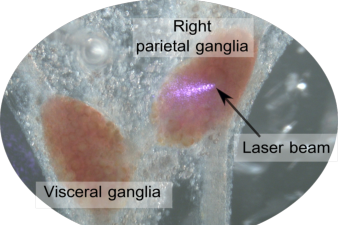
\includegraphics{img/laser/laser-beam.pdf}
	\caption{Illustration of the laser beam focused on a neuron in the right parietal ganglia.}
	\label{fig:laser beam}
\end{wrapfigure} 
The diode laser output was coupled to a single-mode optical fiber to efficiently guide the laser beam to the sample. To adapt the divergence of the laser beam to the fiber optic output, an aspherical lenses-collimator (Thorlabs, F280FC-850) was installed. An achromatic doublet with focal length f=50mm was used to focus the laser beam on the sample (Thorlabs AC127-050-B-ML). The experiments were performed with a laser output power of $\sim$ 90 mW and a power density over the sample of 146 W/cm². The grazing incidence of the laser beam on the sample created a quasi-elliptical spot, with a minor axis of approximately 34{\textmu}m, as shown in Fig. \ref{fig:laser beam}.



The laser was attached to a micro-manipulator (Siskiyou MX160), allowing micrometer precision of the beam placement over the neuron and optimization of the beam focus. The focusing was performed using a binocular microscope (Nikon SMZ-1500) coupled to a CCD camera (XCAM1080PHA, ToupTek Photonics, Zhejiang, China).


\section{Temperature estimation for analyzing laser neuromodulation}
\label{sec:temperature-estimation}
To estimate the CW-NIR laser induced temperature change, we used the open-pipette method employed in previous experimental studies to measure the temperature variation during the illumination \parencite{li_temporal_2013, rabbitt_heat_2016,brown_thermal_2020, brown_response_2021}. We calibrated the resistance and temperature relation using a thermistor (EPCOS, 10$k\Omega$) to measure the temperature in the preparation solution in the range from 23ºC to 29ºC. We used two protocols:  injecting a constant current to calculate the resistance change from the voltage recording, and injecting pulses of a specific current value. From the resulting recording slope of the linear regression, we computed the conversion from voltage to temperature. For the estimation of the temperature change during the laser stimulation, we measured the voltage change during short intervals of laser illumination and the temperature value at its saturation plateau. This estimation is represented in Fig. \ref{fig:temperature estimation}.



\begin{figure}[htb!]
	\centering
	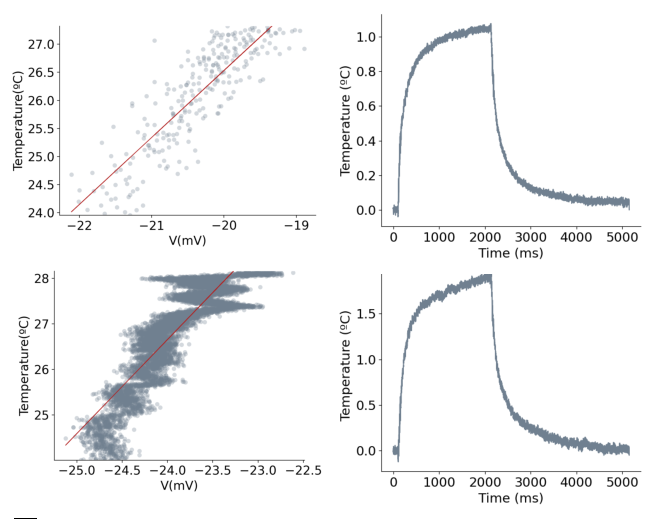
\includegraphics[width=0.8\textwidth]{img/laser/temperature_estimation.pdf}
	\caption{Open-pipette temperature estimation method. Each row in the panel represents pulsed and continuous current delivery for the estimation, respectively. For both examples: left column, temperature and voltage relation. Right column filtered mean of voltage recordings from short illumination intervals in the pipette. }
	\label{fig:temperature estimation}
\end{figure}

